\section{Project Overview and Technology Stack}

\textit{Streamify} is an end-to-end data engineering project that simulates, processes,
and analyses real-time music streaming events.
It transforms raw user interactions — song plays, page views, and authentication events —
into actionable business intelligence through a modern ELT pipeline,
demonstrating how the technologies studied in Chapters 2 and 3 fit together in a
real-world architecture.

\begin{figure}[H]
  \centering
  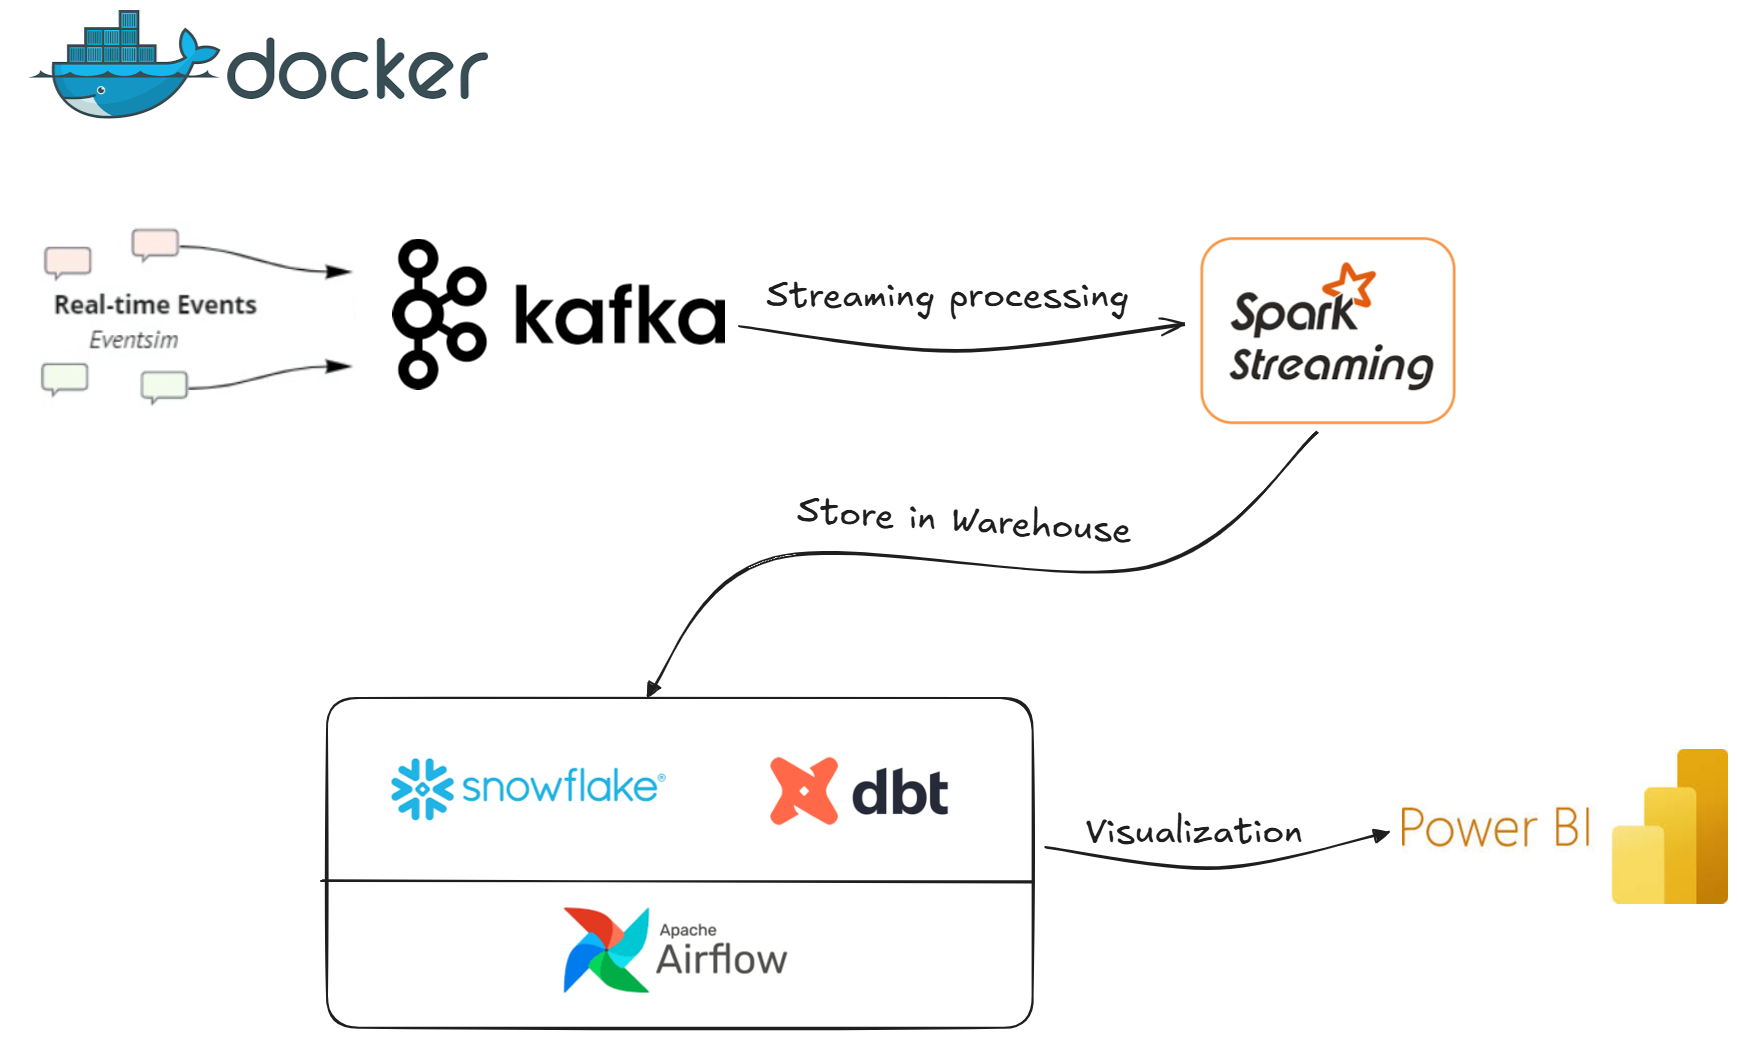
\includegraphics[width=0.92\textwidth]{../image/overview.png}
  \caption{Streamify end-to-end architecture: from event simulation to BI dashboard.}
  \label{fig:streamify-arch}
\end{figure}

The platform is composed of seven layers, each implemented with a best-of-breed open-source
or cloud-native tool:

\begin{table}[H]
  \centering
  \caption{Streamify technology stack.}
  \label{tab:stack}
  \begin{tabularx}{\textwidth}{llX}
    \toprule
    \textbf{Layer}       & \textbf{Tool}              & \textbf{Role} \\
    \midrule
    Data simulation      & Eventsim                   & Generates synthetic music-streaming events based on the Million Songs Dataset. \\
    Message queue        & Apache Kafka (Confluent)   & Durable, partitioned event transport with Schema Registry and Control Center. \\
    Stream processing    & Apache Flink (PyFlink)     & Real-time JSON parsing, timestamp enrichment, and exactly-once sink to Snowflake. \\
    Data warehouse       & Snowflake                  & Cloud-native, elastic analytical storage; receives raw streaming data from Flink. \\
    Transformation       & dbt                        & SQL-based star-schema and wide-table modelling directly inside Snowflake. \\
    Orchestration        & Apache Airflow             & Schedules daily dbt runs via a DockerOperator DAG. \\
    Visualisation        & Power BI                   & Interactive dashboards connected to the star schema in Snowflake. \\
    Containerisation     & Docker Compose             & Single-command reproducible deployment of the full stack on any machine. \\
    \bottomrule
  \end{tabularx}
\end{table}

All services run locally via \texttt{docker compose up --build}.
The Flink Web UI is available at \texttt{http://localhost:8083} and the
Kafka Control Center at \texttt{http://localhost:9021}.
